\documentclass[11pt]{article}
\usepackage[margin=1in]{geometry}
\usepackage{amsmath, amssymb}
\usepackage{booktabs, longtable}
\usepackage{graphicx}
\usepackage{tikz}
\usetikzlibrary{arrows.meta, positioning, shapes.geometric}
\usepackage{listings}
\usepackage{microtype}
\usepackage{placeins}
\usepackage[hidelinks]{hyperref}
\renewcommand{\floatpagefraction}{0.55}
\graphicspath{{generated/}}
\input{generated/macros.tex}

\newcommand{\evsi}{\mathrm{EVSI}}
\newcommand{\evpi}{\mathrm{EVPI}}

\title{voi-rank v1: ranking scenarios by the decision value of a single measurement}
\author{voi-rank pipeline (protocol \voiProtocol, run \voiRunId)}
\date{\today}

\begin{document}
\maketitle

\begin{abstract}
We rank \voiNRanked{} scenarios by the economic value of one measurement sold to
one decision-maker facing one binary decision. Each scenario is scored by the
expected value of sample information (EVSI) of the measurement relative to its
production cost, computed in closed form from seven parameters elicited by a
small language model under a fixed, anchored protocol, with elicitation
uncertainty propagated by Monte Carlo (\voiNDraws{} draws). The primary metric
is \emph{efficiency} $=\evsi/C$: decision value per dollar of measurement.
Because buyer counts and value capture are deliberately out of scope, the
ranking measures per-measurement decision-value density, not business
feasibility.
\end{abstract}

\section{Introduction}

A measurement is a product: someone with a decision to make pays for one
observation because they expect to decide better with it than without it. This
report treats that framing literally. The unit of analysis is a single
\emph{scenario}: one concrete decision-maker (an agent), one binary decision,
one latent binary fact about the world, and one purchasable instrument that
emits one binary signal about that fact. The canonical Bayesian decision
problem then prices the information: how much better, in expected USD, does the
agent do with the signal than without it?

That price is the expected value of sample information (EVSI). Dividing by the
cost $C$ of producing and delivering the measurement gives an efficiency: how
many dollars of decision value one dollar of measurement buys. Ranking many
scenarios by this efficiency is a way of asking: \emph{where in the economy is
a single observation worth the most, per dollar it costs to produce?}

Two design choices keep v1 honest and small. First, everything that would turn
information value into business value --- how many buyers exist, what fraction
of the value a seller can capture, recurrence, rivalry --- is deliberately out
of scope; the interpretation caveat in Section~\ref{sec:limitations} is load-bearing.
Second, all seven parameters per scenario are elicited from a small language
model under a fixed prompt protocol with worked anchor scenarios, repeated
$k=\voiKUsed{}$ times; the elicitation spread is propagated through every
result. The pipeline is an experiment about LLM-based elicitation as much as a
ranking.

\section{Model}
\label{sec:model}

\subsection{Structure}

Latent state $\theta \in \{0,1\}$, with the convention that $\theta = 1$ is the
state in which responding is the correct action. The instrument produces a
binary signal $x \in \{0,1\}$. The agent then chooses an action
$a \in \{0,1\}$ (respond / don't respond); the policy is derived by maximizing
posterior expected utility, never elicited. Utilities are in the regret
parameterization, $u(\theta, a{=}0) = 0$ for both states:
\[
u(1,1) = e\,B, \qquad u(0,1) = -K,
\]
where $B > 0$ is the benefit of a correct response, $K > 0$ the net cost of a
false-alarm response, and $e \in [0,1]$ the action efficacy --- the probability
that the agent actually acts on the signal times the probability that the
action delivers its benefit.

\begin{figure}[ht]
\centering
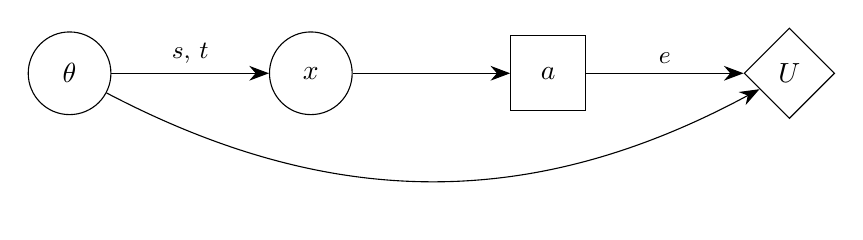
\begin{tikzpicture}[
  node distance=1.6cm and 2.0cm,
  chance/.style={circle, draw, minimum size=1.05cm, inner sep=1pt},
  decision/.style={rectangle, draw, minimum size=0.95cm, inner sep=2pt},
  utility/.style={diamond, draw, minimum size=1.15cm, inner sep=0pt},
  arr/.style={-{Stealth[length=2.5mm]}},
]
\node[chance] (theta) {$\theta$};
\node[chance, right=of theta] (x) {$x$};
\node[decision, right=of x] (a) {$a$};
\node[utility, right=of a] (u) {$U$};
\draw[arr] (theta) -- node[above, font=\small]{$s,\,t$} (x);
\draw[arr] (x) -- (a);
\draw[arr] (a) -- node[above, font=\small]{$e$} (u);
\draw[arr] (theta) to[bend right=28] (u);
\end{tikzpicture}
\caption{Influence diagram. The state $\theta$ (prior $p$) drives the signal
$x$ through sensitivity $s$ and specificity $t$; the agent observes $x$ and
chooses action $a$; utility $U$ depends on $(\theta, a)$, with action efficacy
$e$ discounting the benefit edge.}
\label{fig:influence}
\end{figure}

\subsection{Value of information in closed form}

Write $\pi$ for a belief $P(\theta{=}1)$. Acting optimally at belief $\pi$ is
worth
\[
V(\pi) \;=\; \max\bigl(0,\; \pi e B - (1-\pi) K\bigr),
\]
the maximum over the two actions of posterior expected utility. With signal
probabilities
\[
P_1 = p s + (1-p)(1-t), \qquad P_0 = 1 - P_1,
\]
and posteriors $\pi_1 = p s / P_1$, $\pi_0 = p(1-s)/P_0$ (a branch with zero
probability contributes zero), the value of deciding \emph{with} the signal is
$P_1 V(\pi_1) + P_0 V(\pi_0)$, so
\[
\evsi \;=\; P_1\,V(\pi_1) + P_0\,V(\pi_0) - V(p).
\]

Perfect information replaces the signal with $\theta$ itself: the agent acts
exactly when $\theta = 1$, which is worth $p\,e B + (1-p)\cdot 0$. Hence
\[
\evpi \;=\; p\,eB - V(p)
\;=\; p\,eB - \max(0,\; p\,eB - (1-p)K)
\;=\; \min\bigl(p\,eB,\; (1-p)K\bigr),
\]
using $z - \max(0, z - w) = \min(z, w)$. The two arguments are the expected
regrets of the two ignorant policies: never responding forgoes $p\,eB$;
always responding costs $(1-p)K$. Perfect information is worth exactly the
smaller regret, and $0 \le \evsi \le \evpi$ always.

\subsection{Per-scenario metrics}

On every Monte Carlo draw we compute $\evsi$, $\evpi$, \emph{efficiency}
$= \evsi / C$ (the primary ranking metric, ranked by median), \emph{margin}
$= \evsi - C$, and \emph{headroom} $= \evsi/\evpi$ where $\evpi > 0$ (how much
of the perfect-information value this instrument delivers). Alongside the
ranking we report $P_+ = P(\evsi > C)$ across draws: a high-efficiency
scenario with low $P_+$ is fragile --- its median hides a substantial
probability that the measurement is not worth buying at all.

\section{Method}
\label{sec:method}

\subsection{Elicitation protocol}

Each scenario's seven parameters $(p, s, t, e, B, K, C)$ are elicited from
Claude Haiku via headless CLI calls (version \voiCliVersion), $k=\voiKUsed{}$
independent repeats per scenario. Sampling temperature is not controllable
from the CLI, so \emph{repeats are the noise model}: cross-repeat spread is the
empirical elicitation uncertainty. Calls run in an isolated context (no user
configuration, no tools, a fixed system prompt), so the rendered prompt is the
only input; its SHA-256 hash is stored with every response. The prompt
(Appendix~\ref{app:prompt}) contains, in order: the model definition; two fully
worked anchor scenarios with agreed numbers --- an industrial vibration-survey
decision and an everyday rapid strep test decision --- to pin dollar and
probability scales across scenarios; the scenario under elicitation; and
per-parameter instructions requiring a short reasoning paragraph \emph{before}
the numbers. Each parameter is elicited as (p5, p50, p95) percentiles framed
as ``you would be surprised if the truth fell outside this interval.''
Responses are validated (strict JSON, monotone percentiles, probabilities in
$(0,1)$, positive dollar amounts, an informativeness check
$s_{50} > 1 - t_{50}$, non-degenerate prior); a failed attempt is retried
once, then marked invalid. Validity across all attempts under the final
protocol: \voiValidityRate{} of \voiNAttempts{} attempts. Total elicitation
cost for the final protocol: \$\voiElicitCost.

Scenarios themselves come from two sources: 8 hand-written seeds (doubling as
smoke tests) and a proposer prompt that generates scenarios from ten seed
domains under explicit constraints (one concrete decision-maker; $\theta$ a
checkable binary fact; the instrument a purchasable measurement, not advice;
stakes varied deliberately). No deduplication is applied: scenario text is its
identity.

\subsection{Percentiles to distributions}

Dollar parameters $(B, K, C)$ get lognormal fits; probability parameters
$(p, s, t, e)$ get Beta fits. Fits minimize squared quantile error against the
three elicited percentiles (in log space for lognormals), initialized from
moment matching. Every fit stores its parameters and residual in the database;
badly asymmetric lognormal quantiles and Beta residuals above 0.02 raise a
stored warning flag (\voiFitWarnings{} warnings under the final protocol).
Fits are never recomputed at analysis time.

\subsection{Monte Carlo and sensitivity}

Per scenario, \voiNDraws{} draws (seed \voiSeed) are taken with all seven
parameters independent --- a stated v1 assumption. Where a scenario has $k$
valid repeats, each parameter draws from an equal-weight mixture over the $k$
fitted distributions, so cross-repeat disagreement widens the intervals.
Local sensitivity is the Spearman rank correlation between each parameter's
draws and the efficiency draws, per scenario. Global sensitivity aggregates
$|\rho|$ over the top quartile of the ranking --- the parameters that control
the top of the list are where estimation effort should go next. Rank
stability is computed from the aligned draws directly: the probability that a
scenario ranks in the top 10 by efficiency across joint draws.

\section{Scenario catalog}
\label{sec:catalog}

\input{generated/catalog.tex}

\section{Results}
\label{sec:results}

\input{generated/ranking.tex}

\begin{figure}[ht]
\centering
\includegraphics[width=\textwidth]{fig_ranking.pdf}
\caption{Top 25 scenarios by median efficiency $\evsi/C$. Intervals are
q05--q95 across Monte Carlo draws; dots are medians (open dots: median 0,
shown at the $10^{-3}$ axis floor). The dashed line marks $\evsi = C$:
scenarios to its right buy more than a dollar of decision value per dollar of
measurement.}
\label{fig:ranking}
\end{figure}

\begin{figure}[ht]
\centering
\includegraphics[width=\textwidth]{fig_evsi_vs_cost.pdf}
\caption{Median EVSI against median measurement cost, log--log, with
iso-efficiency diagonals. The top 10 scenarios by median efficiency are
labeled by catalog id. Open dots at the bottom edge are scenarios whose median
EVSI is 0.}
\label{fig:evsi-cost}
\end{figure}
\FloatBarrier

\subsection{Reading the top of the ranking}
\label{sec:commentary}
%% hand-authored from the reasoning strings stored in the DB; numbers via macros
% Commentary on the top of the ranking; written after the final run by
% inspecting the reasoning strings stored in the DB. Numbers via macros only.
(To be written after the final protocol run.)


\FloatBarrier
\section{Sensitivity and elicitation quality}
\label{sec:sensitivity}

\begin{figure}[ht]
\centering
\includegraphics[width=\textwidth]{fig_sensitivity_heatmap.pdf}
\caption{Absolute Spearman correlation between each parameter's draws and the
efficiency draws, per scenario, scenarios ordered by rank.}
\label{fig:heatmap}
\end{figure}

\begin{figure}[ht]
\centering
\includegraphics[width=0.85\textwidth]{fig_headroom.pdf}
\caption{Median headroom $\evsi/\evpi$ against rank. Low headroom at high rank
marks decisions where a better instrument than the current one is worth
building.}
\label{fig:headroom}
\end{figure}

\begin{figure}[ht]
\centering
\includegraphics[width=0.85\textwidth]{fig_rank_stability.pdf}
\caption{Rank stability: probability of membership in the top 10 by
efficiency, across aligned Monte Carlo draws.}
\label{fig:stability}
\end{figure}

\begin{figure}[ht]
\centering
\includegraphics[width=0.85\textwidth]{fig_elicitation_noise.pdf}
\caption{Cross-repeat elicitation noise: spread of the median estimate across
$k=\voiKUsed{}$ repeats, relative to the pooled median, per parameter.}
\label{fig:noise}
\end{figure}

\begin{figure}[ht]
\centering
\includegraphics[width=0.9\textwidth]{fig_top5_densities.pdf}
\caption{Efficiency densities of the top 5 scenarios over positive draws
(log$_{10}$ axis), scaled by $1 - P(\text{eff} = 0)$; the point mass at zero
is the share of draws in which the signal never changes the decision.}
\label{fig:densities}
\end{figure}

Global sensitivity over the top-quartile scenarios puts
$|\rho|$ per parameter at: $p$: \voiGlobalP, $s$: \voiGlobalS, $t$:
\voiGlobalT, $e$: \voiGlobalE, $B$: \voiGlobalB, $K$: \voiGlobalK, $C$:
\voiGlobalC{} --- the ranking's top is controlled chiefly by
\voiGlobalTopParams. Cross-repeat noise over the final run's
$k=\voiKUsed{}$ repeats (median over scenarios of the relative p50 spread;
ranges over five repeats run higher than the matched-$k$ comparison table in
Section~\ref{sec:protocols}) is: $p$: \voiNoiseP, $s$: \voiNoiseS, $t$:
\voiNoiseT, $e$: \voiNoiseE, $B$: \voiNoiseB, $K$: \voiNoiseK, $C$: \voiNoiseC.

\subsection{Protocol comparison}
\label{sec:protocols}

Spearman rank correlations of median efficiency between the latest runs of
each protocol (rows/columns are protocols; the manual column is the
hand-entered seed baseline over its 8 scenarios, and p004 covers only the 17
deepened top-quartile scenarios):

\begin{center}
\input{generated/protocol_compare.tex}
\end{center}

Median cross-repeat spread of the elicited p50, per parameter and protocol,
computed over the first three repeats of each protocol so the comparison is
at matched $k$ (range statistics grow with the repeat count):

\begin{center}
\input{generated/protocol_noise.tex}
\end{center}

%% hand-authored cross-protocol commentary; numbers via macros
% Cross-protocol commentary; written after the protocol iterations.
(To be written after the protocol iterations.)


\FloatBarrier
\section{Limitations}
\label{sec:limitations}

\paragraph{Per-measurement value, not business value.} With value capture and
buyer counts removed by design, the ranking measures how much one observation
is worth to one decision-maker per dollar it costs to produce. A top-ranked
scenario is not a business case: it says nothing about how many such decisions
exist, whether the decision-maker can be reached, or what fraction of the
information value a seller could charge.

\paragraph{Independence.} All seven parameters are drawn independently. In
reality, e.g., high-stakes scenarios ($B$ large) plausibly come with more
expensive instruments ($C$ large) and more careful priors; ignoring the
correlations mostly widens intervals but can also bias efficiency medians.

\paragraph{The efficacy asymmetry.} $e$ multiplies only the benefit branch:
$V(\pi) = \max(0, \pi e B - (1-\pi)K)$. Since $e$ includes the probability
that the agent acts at all, a fully symmetric treatment would discount the
false-alarm cost by the acting probability too; v1 keeps the simpler,
conservative form (it understates the value of acting for noncompliant
agents).

\paragraph{A small model as elicitor.} Haiku is cheap enough to elicit
hundreds of scenario-repeats, but small-model calibration is a real risk. The
mitigations are the two anchors (scale pinning) and $k$ repeats (noise
measurement); Section~\ref{sec:sensitivity} shows the resulting noise levels
per parameter, and the protocol-comparison matrix shows how much the ranking
moves when the prompt changes. Both are evidence about --- not proof of ---
elicitation quality. The hand-entered seed baseline correlates with the final
protocol's ranking at $\rho = \voiRhoManual$ over \voiRhoManualN{} shared
scenarios.

\paragraph{Selection effects of validation.} The informativeness check
($s_{50} > 1 - t_{50}$) rejects elicitations rather than repairing them; a
scenario whose instrument haiku consistently sees as uninformative drops out
of the ranking instead of appearing with $\evsi \approx 0$.

\paragraph{Deferred by design.} Capture fraction, number of buyers,
annualization and recurrence, rivalry, compliance or stamp demand, risk
aversion, parameter correlations, retrodiction validation, richer state and
signal spaces (POMDPs), and deduplication are all out of scope for v1.

\section{Learnings}
\label{sec:learnings}

%% hand-authored, distilled from LEARNINGS.md after protocol iterations
% Distilled from LEARNINGS.md after the protocol iterations.
(To be written after the protocol iterations.)


\appendix

\section{Elicitation prompt template}
\label{app:prompt}

The exact template of the final protocol (placeholders \texttt{\$title},
\texttt{\$agent}, \texttt{\$decision}, \texttt{\$theta\_definition},
\texttt{\$instrument} are substituted per scenario):

\lstinputlisting[basicstyle=\scriptsize\ttfamily, breaklines=true,
                 frame=single, breakindent=0pt]{../elicitation/templates/elicitor.md}

\section{Reproduction}
\label{app:repro}

Everything downstream of the elicitation database is deterministic given the
stored seed (run \voiRunId: seed \voiSeed, \voiNDraws{} draws, code revision
\texttt{\voiCodeHash}). The database stores every prompt hash, raw model
response, fitted distribution, and run configuration; figures and tables in
this report are generated exclusively from it. See \texttt{README.md} in the
repository root for the run order.

\end{document}
